\documentclass[a4paper,twoside]{article}

\usepackage{epsfig}
\usepackage{amssymb}
\usepackage{amstext}
\usepackage{amsmath}
\usepackage{amsthm}
\usepackage{multicol}
\usepackage{pslatex}
\usepackage{apalike}
\usepackage{SCITEPRESS}


\usepackage{listings}
\usepackage{xcolor}
\usepackage{subfig}
\usepackage{graphicx}
\usepackage{epstopdf}
\usepackage{flushend}
\usepackage{listings}
\usepackage{color}
\usepackage{multicol}
\usepackage{amsmath}
\usepackage{stfloats}


\usepackage{floatrow}

\colorlet{punct}{red!60!black}
\definecolor{background}{HTML}{EEEEEE}
\definecolor{delim}{RGB}{20,105,176}
\colorlet{numb}{magenta!60!black}

\lstdefinelanguage{json}{
    basicstyle=\scriptsize\ttfamily,
    numbers=none,
    numberstyle=\scriptsize,
    stepnumber=1,
    numbersep=8pt,
    showstringspaces=false,
    breaklines=true,
    frame=none,
    backgroundcolor=\color{background},
    literate=
     *{0}{{{\color{numb}0}}}{1}
      {1}{{{\color{numb}1}}}{1}
      {2}{{{\color{numb}2}}}{1}
      {3}{{{\color{numb}3}}}{1}
      {4}{{{\color{numb}4}}}{1}
      {5}{{{\color{numb}5}}}{1}
      {6}{{{\color{numb}6}}}{1}
      {7}{{{\color{numb}7}}}{1}
      {8}{{{\color{numb}8}}}{1}
      {9}{{{\color{numb}9}}}{1}
      {:}{{{\color{punct}{:}}}}{1}
      {,}{{{\color{punct}{,}}}}{1}
      {\{}{{{\color{delim}{\{}}}}{1}
      {\}}{{{\color{delim}{\}}}}}{1}
      {[}{{{\color{delim}{[}}}}{1}
      {]}{{{\color{delim}{]}}}}{1},
}

\newcommand{\specialcell}[2][c]{%
  \begin{tabular}[#1]{@{}l@{}}#2\end{tabular}}


\lstset{breaklines=true}

\begin{document}

\title{MoBio\subtitle{A mobile application for collecting data from sensors} }

\author{\authorname{Petr Je\v{z}ek\sup{1} and Roman Mou\v{c}ek\sup{1}}
\affiliation{\sup{1}New Technologies for the Information Society,
              Department of Computer Science and Engineering,
              Faculty of Applied Sciences,
              University of  West Bohemia,
              Univerzitn\'{i} 8,
              306 14  Plze\v{n},
              Czech Republic}
\email{jezekp@ntis.zcu.cz, moucek@kiv.zcu.cz}
}

\keywords{MoBio, sensor, Android, mobile application, brain data, health data, domain terminology, data transfer, EEGBase}

\abstract{There are a lot of sensors for monitoring human health and/or fitness level on the market. They facilitate collection of data from the human body and advanced devices even facilitate data transfer to remote servers where the collected data are further processed. While health data, obtained e.g. from accelerometers or chest straps, are collected rather frequently, brain electrophysiology data, obtained from surface electrodes, are still collected relatively rarely. However, integration and correlation of brain signals with other sensory data would be very interesting for next research of physical and mental health. Although capturing brain signals in real environment still faces technological difficulties, current development of common infrastructure seems to be useful. Then this article deals with various architectures and data formats used for storage and transfer of sensory data and their possible integration with existing neuroinformatics approaches. As a~solution we introduced a~terminology describing data from a~limited collection of sensors. The terminology is implemented in the odML format and integrated in a~proof-of-concept Android application. Data transfer, storage and visualisation as well as integration with a~remote neuroinformatics resource are presented.}

\onecolumn \maketitle \normalsize \vfill

\section{\uppercase{Introduction}}
\label{sec:introduction}

\noindent
There are a lot of factors affecting human health. Some of them such as genetics, environmental influence or internal state of an individual cannot be easily measured. On the other hand, there are the factors such as blood pressure, glucose level or heart rate that can be measured relatively easily and non-invasively using cheap sensors. For a long time electrophysiological measurements have been conducted in laboratories equipped by common desktop computers and non-transferable measuring devices. Fortunately, this situation has been rapidly changing. One of the reasons is increasing popularity of smart devices such as smart-phones or tablets. According to eMarketer \cite{emark} two billion people will own a smart-phone in 2016. Simultaneously, a lot of relatively cheap sensors for measuring potentials from the human body are available on the market. The data produced by these sensors are usually transferred wirelessly, consequently they can be read and processed by smart devices. This technical progress enables a particular shift of treatment from hospitals to home environments and facilitates collecting data during outdoor activities. The obtained data can be used in two fundamental intersecting ways.

At first, assistive technology approach serves to stimulate, maintain, and improve functional capabilities of people with special needs including disabled people or aging population. Getting independence and self-sufficiency increases the quality of life in general.

The second approach is focused on sportsmen or actively living people. People are being monitored when they are performing specific activities (e.g. running or long distance walking). The data are used for a long term monitoring of their fitness level.

So far we have not talked about a significant source of electrophysiology data, the human brain. Although there are technological improvements for capturing surface brain data in real environment, this kind of data collection is still not widespread. However, integration and correlation of brain signals with other sensory data would be very interesting for next research of physical and mental health. 

Our research group operates a completely equipped laboratory~\cite{10.3389/fninf.2014.00020} for electrophysiological measurements. We are focused mainly on experimental work using the methods and techniques of electroencephalography (EEG) and event-related potentials (ERP). Except of the permanent laboratory we also operate a mobile laboratory equipped by a set of laptops and portable measuring devices for performing experiments in the external environment. With advancing efforts to extend the laboratory to collect diverse collections of data (e.g. blood pressure, glucose level, heart rate) we are extending our infrastructure (hardware devices and software tools) to support  measurements of heterogeneous data from various kinds of sensors.

In this paper we deal with deals with various architectures and data formats used for storage and transfer of sensory data and their possible integration with existing neuroinformatics approaches. Since data from existing sensors are usually stored in proprietary formats and transferred to closed databases, it is difficult to use them in experimental laboratories. As a~solution we introduce a~terminology describing data from a~limited collection of sensors. Then a~prototype of a mobile client for collecting data from these sensors is presented. This client provides integration with a limited set of devices and enables data to be transferred and visualized in a remote storage.

\section{\uppercase{state of the art}}
\label{sec:state-of-the-art}

\noindent
According to \cite{Lowe2012242} applications using sensors can be divided into three categories. The first category, Smart Phone Applications, use either GPS or 
on-board kinematic sensors as the technologies of choice for monitoring exercise. The second category comprises of any system that uses a~central controller
and an external sensor. The last category comes from image processing domain. It uses a combination of a computer screen and a camera. The camera monitors the exact movement and position of the entire body during exercise. The screen is used for the interaction with the user.

The first category represents applications such as Endomondo or Runkeeper. The second category is represented by e.g. Nike+, miCoach, Garmin Heart Belt or Fora Active tonometer. A~typical representative of the third category is Microsoft Kinect. While Microsoft Kinect is designed for the indoor use, all other devices are designed mostly for the outdoor use.

Available tools and sensors are usually designed for one specific activity. They are able to record only limited variety of data. In addition, due to their proprietary structure they do not provide suitable interfaces for integration with other systems.

As well as other communities neuroinformatics community identified problems with a long-term description, storage and management of experimental data/metadata \cite{CRCNS}. To facilitate solution of these difficulties International Neuroinformatics Coordinating Facility (INCF) \cite{INCF} covers activities for development of infrastructures and data standards in neuroinformatics community. Ontology for Experimental Neurophysiology (OEN) \cite{10.3389/conf.fninf.2014.18.00044} uses semantic web approach to describe terminology used in biomedical science and neuroscience. Our research groups developed a~system for long term storage and management of EEG/ERP experimental data and metadata, EEGBase \cite{ISI:000306821100004} that was recently extended by a system of templates suitable for storing various data and metadata structures. A mobile EEGBase client \cite{10.3389/conf.fninf.2013.09.00046} is a supplementary Android tool that enables collecting experiments out of the laboratory and provides an on-line synchronization with EEGBase.


\section{\uppercase{Sensor Architectures and Data Transfer}}
\label{topology_data_transfer}

\noindent
Sensors use different ways to manipulate data. Some sensors have their own displays or internal memories for storing measured data that can be later transferred to a long term storage. These devices usually provide a complete history (of course, limited by the capacity of their internal memories) of stored measurements. On the other hand, devices such as heart rate meters do not have any internal memory. Data can be transferred only at the time of measurement. According to the way the data are distributed, we defined three levels of sensor architecture.

\begin{itemize}
 \item one-layer - The sensor is a stand-alone unit having a display, memory, and a set of controls. Such a sensor is completely self-controlled and does not establish any connection to a~remote system.
 \item two-layers - The sensor captures data that are finally sent to a remote system (the sensor may/may not have an internal memory). This remote system can be a common computer/laptop or a smart phone/watch etc.
 \item three-layers - A cloud service is added to the two-layer architecture. The captured data are sent to a~remote server where they are stored, managed, and analyzed.
\end{itemize}

 A lot of sensors belonging to the one-layer architecture, including various glucometers, tonometers, and step counters, store captured data in a proprietary storage. These devices usually do not require/provide any connection to other systems. Representatives of two-layer architecture include sensors such as heart rate belts or  step counters. They often do not have their own display and usually use Bluetooth or ANT (resp ANT+)\footnote{ANT is the protocol while ANT+ is a set of mutually agreed definitions what the information sent over ANT represents.}technologies  for data transfer. Data are usually displayed on a screen of a smart device. Because of the limited performance of mobile devices only a basic data processing is provided. Advanced data processing is performed on a remote server that forms part of the three-layer architecture. There are few exceptions such as BlibCare tonometer equipped with WiFi. Then the captured data can be transferred directly by using e.g. a home WiFi network.



\section{\uppercase{Tested systems}}
\label{tested_systems}
\noindent

E-health and fitness systems that use the three-layer sensor architecture described above are most suitable for long term storage and management of collected data. When providing a remote data transfer to a~server, these devices are also suitable to be integrated with neuroinformatics infrastructures. The biggest obstacle encountered is usually a~data format of transferred data. When devices implement Bluetooth or ANT+ technologies, they can use a lot of defined profiles including Blood Pressure Profile (BLP), Heart Rate Profile (HRP), Health Thermometer Profile (HTP)\footnote{https://developer.bluetooth.org/TechnologyOverview/ Pages/Profiles.aspx} for Bluetooth, or Weight Scale and Heart rate\footnote{https://www.thisisant.com/developer/ant-plus/device-profiles} for ANT+.

Table~\ref{tab:tested_systems} summarizes and provides evaluation of the e-health and fitness systems we tested. Only the systems providing at least a~cloud service as a~storage or statistical results as an analytic result were selected. For all systems we considered the number of supported internal (e.g. a GPS sensor on a~smart phone) and external sensors. This number is very limited as can be seen in Table~\ref{tab:tested_systems}. Two systems do not support any sensor; data are inserted manually. The last column \emph{Design} is a~subjective evaluation of the user interface. Although all tested systems use the ANT or Bluetooth technology, they implement a proprietary transfer format instead of using any available profile.


\begin{table*}[t]
\centering
\caption{Tested e-health and fitness systems}
\label{tab:tested_systems}
\begin{tabular}{|l|c|c|c|c|c|c|c|}
\hline
               & \multicolumn{1}{l|}{\begin{tabular}[c]{@{}l@{}}Intern.\\  sensors\end{tabular}} & \multicolumn{1}{l|}{\begin{tabular}[c]{@{}l@{}}Extern.\\ sensors\end{tabular}} & \multicolumn{1}{l|}{\begin{tabular}[c]{@{}l@{}}Conti-\\nuous\\  measure-\\ments\end{tabular}} & \multicolumn{1}{l|}{\begin{tabular}[c]{@{}l@{}}Single\\  measure-\\ments\end{tabular}} & \multicolumn{1}{l|}{Statistics} & \multicolumn{1}{l|}{\begin{tabular}[c]{@{}l@{}}Cloud\\ Service\end{tabular}} & \multicolumn{1}{l|}{Design} \\ \hline

 \specialcell{Endomondo\\  \textit{www.endomondo.com}}     & 2                                                                                & 3                                                                               & \textbullet                                                                                        &                                                                                     & \textbullet                                & \textbullet                                  & +                           \\ \hline
\specialcell{Runstatic \\ \textit{www.runtastic.com}}      & 2                                                                                & 2                                                                               & \textbullet                                                                                        &                                                                                     & \textbullet                                & \textbullet                                 & +                           \\ \hline
\specialcell{Pedometer \\ \textit{ www.runtastic.com}\\ \textit{/en/apps/pedometer}}      & 1                                                                                &                                                                                 & \textbullet                                                                                        &                                                                                     & \textbullet                                & \textbullet                                  & -                           \\ \hline
\specialcell{Push-ups \\ \textit{www.runtastic.com/} \\ \textit{en/apps/pushups}}       & 1                                                                                &                                                                                 & \textbullet                                                                                        &                                                                                     & \textbullet                                & \textbullet                                  & +                           \\ \hline
\specialcell{Heart rate \\ \textit{www.runtastic.com}\\ \textit{/en/apps/heartrate}}     & 1                                                                                &                                                                                 &                                                                                         & \textbullet                                                                                    & \textbullet                                & \textbullet                                  & +                           \\ \hline
\specialcell{Sport Tracker \\ \textit{www.sports-tracker.com}}  & 1                                                                                & 2                                                                               & \textbullet                                                                                        &                                                                                     & \textbullet                                & \textbullet                                  & +                           \\ \hline
\specialcell{Health Tracker \\ \textit{play.google.com/store/apps/} \\ \textit{details?id=com.benoved.phr\_lite}} &                                                                                  &                                                                                 &                                                                                         &                                                                                     & \textbullet                                &                                   & -                           \\ \hline
\specialcell{Madbarz \\ \textit{madbarz.com}}        &                                                                                  &                                                                                 &                                                                                         &                                                                                     & \textbullet                                & \textbullet                                  & +                           \\ \hline
\specialcell{eVito \\ \textit{www.evito.cz}}        & 1                                                                                 & 5                                                                                  & \textbullet  & \textbullet                                                                                      &  \textbullet                                                                                   & \textbullet                                                                & +                           \\ \hline
\end{tabular}
\end{table*}


\section{\uppercase{Mobile application prototype}}
\label{mobile_app_prototype}


\subsection{System Scope}

Having difficulties with closed-source dedicated devices we present a prototype of a mobile application that solves the issues described above. It aggregates data from various sensors into a~flexible data storage on the server. The data can be used by human reader or processed by automatic readers. The application can be easily used outdoors and in areas without Internet connectivity. When the client gets on-line, the stored data are synchronized with EEGBase (contrary to the original purpose EEGBase is newly considered as a storage and management system for any kind of electrophysiology data). However, the main core of this solution is a~proposal and implementation of suitable terminology for sensory data.

\subsection{Format Selection}

Since the aim of the application is to support large collections of sensors, it must store data in a flexible data format. Existing data formats are based on different levels of abstraction and include low-level binary formats, highly abstract implementation-independent data formats, and formats based on ontologies. We required a~format that provided a sufficient level of abstraction to be system independent, but also easy-to-use format having no specific demands on users. Having been involved in neuroinformatics community and having been persuaded that the similar solution could be used for other sensory data, we preferred open-source formats supported and accepted in this domain.

The working group of the INCF Task Force on Electrophysiology\footnote{http://www.incf.org/programs/datasharing/ electrophysiology-task-force} introduced two approaches towards defining a standard, which may eventually be merged \cite{10.3389/conf.fninf.2013.09.00069}. The first one uses the Hierarchical Data Format (HDF5) \cite{hdf5} or respectively epHDF, the  specialized HDF5 format for electrophysiology. The NIX format~\cite{Stoewer:2014} provides a data model for storing experimental data in HDF5, together with metadata in the odML format~\cite{10.3389/fninf.2011.00016}. We selected odML (odML is a~free form tree-like structure of sections, properties and values) as a suitable format for the presented application because of its platform-independence, simplicity, and human-readability. Moreover, it ensures a compatibility with other systems developed in neuroinformatics community, for example \cite{10.3389/conf.fninf.2014.18.00029}, \cite{10.3389/conf.fninf.2014.18.00053}, and~\cite{10.3389/conf.fninf.2013.09.00025}.

\begin{figure}
  %\vspace{-0.2cm}

  \centering
   {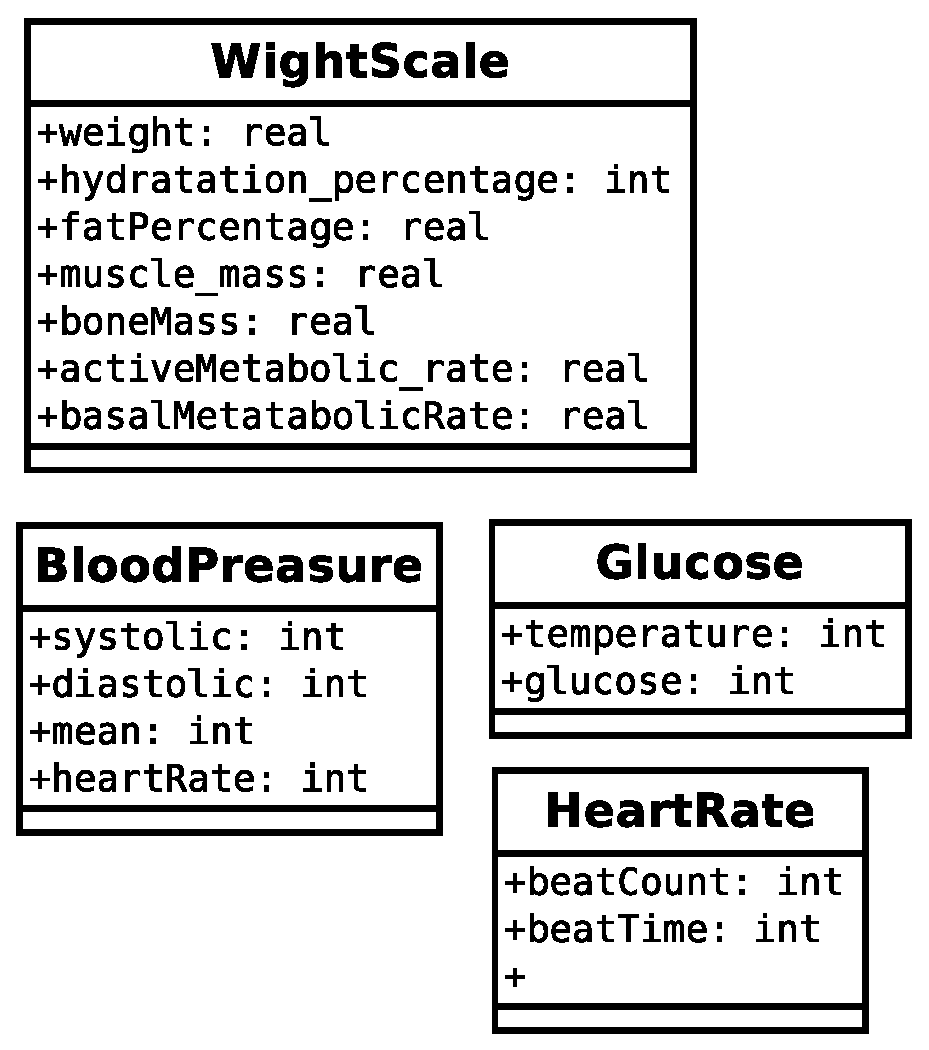
\epsfig{file = Materials/terminology.eps, width = 7cm}}
  \caption{Proposed Terminology}
  \label{fig:Terminology}
 \end{figure}


\subsection{Terminology}

Figure~\ref{fig:Terminology} shows a~terminology based on the odML format and proposed for measurements of blood pressure, heart rate, glucose level, and weight scale including hydratation, muscle mass or bone mass. Listing~\ref{odml_example} shows a JSON representation of the blood pressure data structure, the section \emph{blood\_presure} with properties \textit{systolic\_pressure}, \textit{diastolic\_pressure}, \textit{mean\_pressure}, and \textit{heart\_rate} are defined. The document is simplified to keep readability. A~complete document contains a~complete set of properties describing the experiment. Because of the flexibility of the odML format, this terminology can be easily extended for other measurements.

\begin{lstlisting}[language=json,caption=Blood pressure example, label=odml_example]
{
     "metadata":{
         "odML":{
            "date":"2015-07-03",
            "xmlns:gui":"http://www.g-node.org/guiml",
            "section":[
               {
                  "name":"blood_pressure",
                  "property":[
                     {
                        "name":"systolic",
                        "value":{
                           "type":"int",
                           "content":80
                        },
                     },
                     {
                        "name":"dyastolic",
                        "value":{
                           "type":"int",
                           "content":60
                        },
                     },
                        "name":"mean",
                        "value":{
                           "type":"int",
                           "content":70
                        },
                     },
                     {
                        "name":"heart_rate",
                        "value":{
                           "type":"int",
                           "content":52
                        },
                     },
                  ],
                  "type":"blood_preasure"
               }
            ],
            "version":1
         }
}
\end{lstlisting}

\subsection{Architecture and Implementation}

To support the use of open source technologies we implemented the MoBio application for the Android platform that is available on a~wide range of devices including tablets and mobile phones  (according to StatCounter\footnote{http://gs.statcounter.com} more than 60\% of devices are operated by Android). Moreover, there are other advantages to use this platform, for example a~lot of cheap devices on the market, large community of developers, and easy publication of applications.

Figure \ref{fig:Architecture} shows the used architecture. The user collects data using a body sensor. The data are transferred to MoBio running on a smart phone using an~ANT+ or Bluetooth profile. Then MoBio transfers data expressed in an odML terminology to the server.

The presented proof of concept implementation provides basic functionality including management of user accounts, support for a limited set of sensors, and visualization of stored data. Collected data are stored on a~SD card and can be visualized directly on the mobile phone screen or transferred to the server and stored there for future processing. The registration form includes both basic information about the user such as his/her name or email and advanced information such as gender, weight, height, current fitness level, etc. All these data are required because they can affect results of measurements.

Supported devices must enable either Bluetooth or ANT transfer. In the current implementation we successfully tested a~limited set of devices produced by Garmin and Fora producers. When the device is paired, the user can transfer data. Figure~\ref{fig:mob_app_prev} shows a basic functionality provided to the logged user. Figure~\ref{fig:capture_a} shows a~list with a~paired device, the Garmin Heart Rate Sensor. The current heart rate is shown in Figure~\ref{fig:capture_b}. When the user starts a measurement, data are continuously stored in the device and the related heart rate chart is continuously plotted as shown in Figure~\ref{fig:capture_c}.

 \begin{figure}
  %\vspace{-0.2cm}

  \centering
   {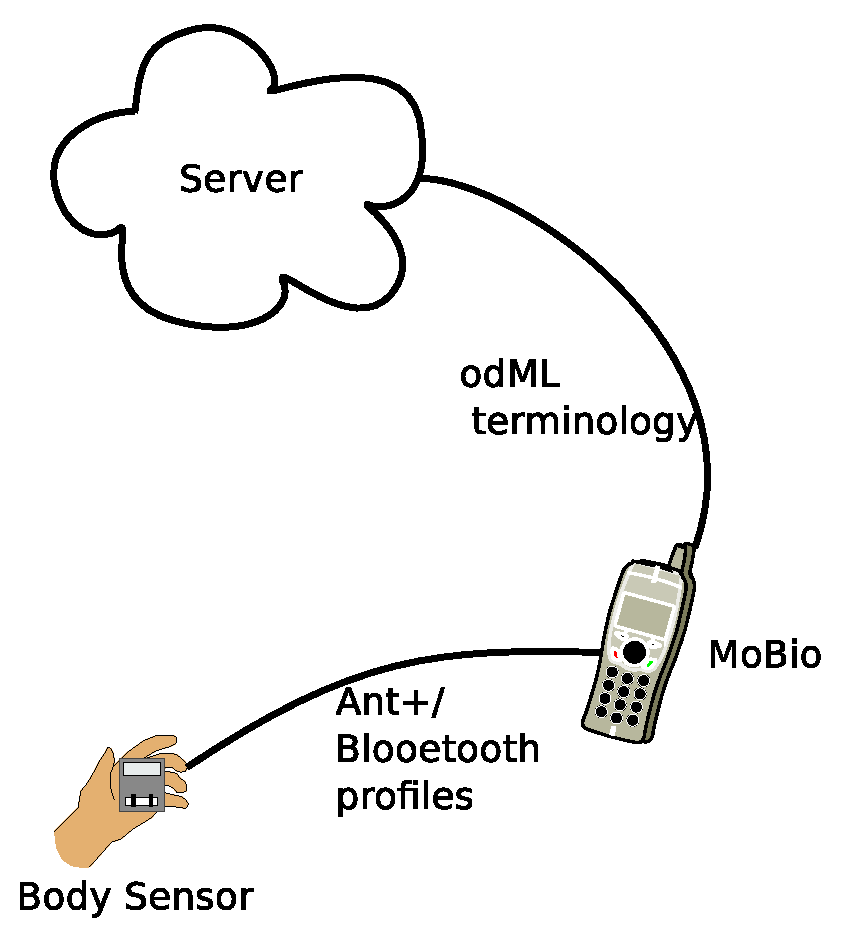
\epsfig{file = Materials/architecture.eps, width = 7cm}}
  \caption{MoBio System Architecture}
  \label{fig:Architecture}
 \end{figure}

\begin{figure*}[!ht]
% Use the relevant command to insert your figure file.
% For example, with the graphicx package use
\begin{tabular}{c}
\subfloat[List of available sensors]{\includegraphics[width = 4cm, height=6.0cm]{Materials/Capture.PNG}\label{fig:capture_a}}
\hspace{10pt}\subfloat[Current heart rate]{\includegraphics[width = 4cm, height=6.0cm]{Materials/Capture3.PNG}\label{fig:capture_b}}
\hspace{10pt}\subfloat[Long term heart rate]{\includegraphics[width = 4cm, height=6.0cm]{Materials/Capture2.PNG}\label{fig:capture_c}}
\end{tabular}
% figure caption is below the figure
\caption{Mobio Application Preview}
\label{fig:mob_app_prev}
\end{figure*}


\begin{figure}
  %\vspace{-0.2cm}

  \centering
   {\epsfig{file = Materials/portal_example2.png, width = 7cm}}
  \caption{Data stored in EEGBase}
  \label{fig:EEGBase}
 \end{figure}


\subsection{Integration with EEGBase}

The collected data can be transferred to any storage system supporting the odML format. EEGBase, extended with an advanced system of user templates for storing various kinds of data and metadata in the odML format, was selected as a~storage. Any template can be defined according to data coming from a sensor and enriched by a~relevant set of metadata.

Technically EEGBase provides a RESTful API containing methods for uploading newly collected data. The user can select an automatic data upload triggered when the user gets on-line. The user can also enforce the upload manually. Once the data are transferred to the server, the odML document is stored in the ElasticSearch noSQL database and visualized. Figure~\ref{fig:EEGBase} shows visualization of the data from Listing~\ref{odml_example}.


\section{Discussion}
Presented terminology covers basic set of sensors. Moreover it is easy extensible because of the open format odML. Its JSON serialization is suitable for wireless transfer because of low memory requirements in comparison with e. g. XML.  If we suppose a large sensor network (say 15 for human tracking) with 10 signals per sensor and say sampling frequency 50Hz, and if one sample produces 1B of the data then the one hour record produces about 27MB of data plus a few kilobytes of space for JSON elements. It will work without difficulties with regard to the capacity of todays SD cards. The data security is ensured by used protocols because both Bluetooth and ANT support the data transfer via a secured channel.

\section{\uppercase{Conclusions}}
\label{sec:conclusion}

\noindent
We observed a diverse collection of available sensors on the market. These sensors vary e.g. in the used data format and data transfer protocol. We identified architectures reflecting the ways the data collected from sensors are managed. Then we selected the three-layer sensor architecture as the most suitable one for the long-term storage and processing of sensory data. Since sensors producers use their own systems and proprietary data formats, there are difficulties with reading, transferring and processing data. As a solution we presented a prototype of a custom terminology describing data collected from sensors. This terminology is implemented in the Android mobile system that serves as a proof-of-concept implementation supporting a~limited set of sensors. Then a~complete process from collecting data by the mobile system, storage of data in a universal format respecting presented ontology and final storage of data in EEGBase is outlined.

Our future work includes extension of the presented terminology to cover a~broader collection of health sensors. Then the extended mobile application will convert the data transferred using Bluetooth or ANT+ profiles to an odML document that satisfies this terminology. The described data can be fully managed in the systems such as EEGBase. A new version of EEGBase with the support of the presented terminology and description of the complete terminology itself will be released. This terminology may well serve to developers of similar systems when they want to collect and process data from health sensors.


\section*{\uppercase{Acknowledgements}}

\noindent

Will be added in CR version


\vfill
\bibliographystyle{apalike}
{\small
\bibliography{citations-ic4awe-2016,frontiers,bibliography,neuroportals}


\vfill
\end{document}

